\documentclass[11pt,a4paper]{book}
\usepackage{amsmath}
\usepackage{amssymb}
\usepackage{enumitem}
\usepackage{amsthm}
\usepackage{MnSymbol}
\setlength{\parindent}{0pt}
\usepackage[utf8]{inputenc}
\usepackage{listings} [python]
\usepackage{hyperref}
\usepackage{tikz}
\usetikzlibrary{arrows.meta}
\usetikzlibrary{arrows}


\newtheorem{theorem}{Theorem}[section]
\newtheorem{corollary}{Corollary}[theorem]
\newtheorem{lemma}[theorem]{Lemma}

\theoremstyle{definition}
\newtheorem{definition}{Definition}[section]

\theoremstyle{definition}
\newtheorem{example}{Example}[section]

\theoremstyle{definition}
\newtheorem{cexample}{Causality Example}[section]

\theoremstyle{remark}
\newtheorem*{remark}{Remark}



%\theoremstyle{definition}
%\newtheorem{example}{Example}[section]

%opening
\title{Thesis\\
\author{Konstantin Kueffner}}


%\newcommand{\imp}[1]{$\supset$}


\newcommand{\interi}{\mathcal{I}}
\newcommand{\interj}{\mathcal{j}}

% Graph Theory

\newcommand{\gtpred}{\mathcal{N}^+}
\newcommand{\gtsucc}{\mathcal{N}^-}
\newcommand{\gtdegpred}{\deg^+}
\newcommand{\gtdegsucc}{\deg^-}



% Neuron Diagram
\newcommand{\ngraph}{\mathcal{G}}
\newcommand{\ndiagram}{\mathcal{D}}




% Causal Modelling

\newcommand{\cmodel}{\mathcal{M}}
\newcommand{\csig}{\mathcal{S}}
\newcommand{\cfoos}{\mathcal{F}}
\newcommand{\crange}{\mathcal{R}}

\newcommand{\cvars}{\mathcal{W}}
\newcommand{\cenvars}{\mathcal{V}}
\newcommand{\cexvars}{\mathcal{U}}
\newcommand{\crel}{\mathcal{E}}
\newcommand{\cbinfoos}{\mathbb{F}_{\mathbb{B}}}


\usepackage{biblatex}
\addbibresource{references.bib}


\begin{document}

\maketitle

\chapter{Introduction}


\section{Preliminaries}

\subsection{Graph Theory}  
A directed graph $G$ is the pair $(V,E)$ with $V$ being a set of vertices and $E \subset V\times V$ being a set of edges. For $v,w \in V$ $v$ is a \emph{direct predecessor} of $w$  iff there exists $(v,w) \in E$; $y$ is a direct successor of $w$ iff $(w,v) \in E$. For $v \in V$, $\gtpred(v)$ is the set of direct predecessors of $v$; $\gtsucc(v)$ is the set of direct successor of $v$; $\gtdegpred(v):= |\gtpred(v)|$ is the in-degree of $v$; $\gtdegsucc(v):= |\gtsucc(v)|$ is the out-degree of $v$. A vertex $v\in V$ is called a sink \emph{sink} if it has no successors, i.e.\ $\gtsucc(v) = \emptyset$ and a \emph{source} if it has no predecessors, i.e.\ $\gtsucc(v) = \emptyset$.
% If $E$ is a total ordered set of edges with respect to $\preceq$ then for some $v\in V$, $\gtpred(v)$ and $\gtsucc(v)$ are tuples constructed based on the ordering of the edges, i.e. $\gtpred(v):=(v_1, \dots , v_n)$ such that for $i < j \leq n$, $(v_i,v) \prec (v_j,v)$ and analogue for $\gtsucc(n)$. 



A path (XXXXX)


\paragraph{Exogenous and Endogenous} Variables, denoted by $\cvars$, can be used for describing the state of the world. However, often it is useful to partition those variables into two groups, i.e. exogenous and endogenous variables. \emph{Exogenous} variables, denoted by $\cexvars$, are variables whose values are determined by factors outside of the model. Whereas \emph{endogenous}, denoted by $\cenvars$ variables are determined by the values of exogenous variables based on the rules relating variables within the model. 




\chapter{Causation}
Before venturing forward into the analysing some of the many formalisms concerned with the notion of causality, a small detour through the philosophical neighbourhood of the literature landscape is necessary. 
That is, the notion of causality has enchanted humanity since the inception of philosophy, thus it would be criminally negligent to gloss over centuries of discussion and enquiry.  
Especially, since an investigation, even a small one, into the various traditions and approaches to causation in the philosophical literature provides additional context for the more computationally minded approaches discussed in 
Chapter \ref{ch:comp_causality}. In this particular case, it serves as a foundation from which the fist classification scheme for formalisms is erected. 
Moreover, when discussing (mostly) rigorously defined formalisms one needs a measure of aptitude.  Unfortunately, as of now it seems that the best method for assessing the capabilities of a formalism is by running it against an array of examples, each trying to cover some pitfall of causal reasoning. In Chapter \ref{ch:comp_causality}, those examples will be used as a second classification scheme. 
Therefore, the chapter will be structured as follows. Section \ref{sec:causation:approaches_to_causation} relies heavily on \cite{beebee2009oxford} and provides a brief overview over the history of and the approaches to causation from a philosophical point of view. Section \ref{sec:causation:examples} is presents a collection of examples used to capture the peculiarities of human (actual) causal inference and discusses their relationships. 
Finally, Section \ref{sec:causation:classify_causation} proposed a schemata for classifying formalisms  with

\section{Approaches to Causation}
\label{sec:causation:approaches_to_causation}
According to \cite{beebee2009oxford} there are standard and alternative approaches to causation. The prior including regularity theories, counter-factual theories, probabilistic theories, causal process theories and agency interventionist theories, while the latter includes theories about causal power and capacities, an anti-reductionist approach, the field of causal modelling, an approach requiring the existence of causal mechanism and one that embraces pluralism. Moreover, in \cite{halpern2016actual} distinguishes between two separate notions of causality, i.e. type (or general) causality and token (or actual) causality. 


\subsection{Type and token causality} i
The classification of causality into type and token causality is rooted in the metaphysical distinction between types and tokens, which is used to differentiate a general sort of thing and its particular occurrence \cite{wetzel2018typetoken}.

\begin{example}[\cite{hausman2005causal}]
Consider the statement 
\begin{quote}
Rose is a rose is a rose is a rose.
\end{quote}
How many different words does this sentence have.  Depending on what one may understand as word, this sentence contains three or ten different words. In the prior, the word-types of the sentence are counted, while in the latter the word-tokens are counted. 
\end{example}

This distinction, can be used to distinguish two (possibly distinct) notions of  causality. \emph{Type causality}, is concerned with forward looking statements such as ``smoking causes lung cancer'', granting their wielder some predictive capabilities. Hence, establishing type causality is often the pursuit of scientific enquiry. However, often type-causal relations do not establish a strong causal connection, but rather a causal tendency. Meaning, while smoking may cause lung cancer, it is not necessary the case that a smoker will develop lung cancer, thus one may be better suited with the statement ``smoking tends cause lung cancer''. By contrast, if one wants to establish that the act of smoking caused lung cancer in a particular person, one speaks of token causality. Meaning \emph{token causality} tries to establish a connection between events that explains a certain outcome arose, thus it tends to be backwards looking.
Unfortunately, it does not seem clear whether those two notion of causation are distinct; whether type causation is merely a generalisation token causal relations, which are assumed to be fundamental, whether token causation is merely an instantiation of type level laws, which are considered as the fundamental element; whether type and token causality are simple different expression of a singular causal relation. 
For example, as will be observed in Chapter \ref{ch:comp_causality},  Halpern defines token causality in terms of type causal statements \cite{hausman2005causal,halpern2016actual}. 


The debate of what constitutes token or type causality can be extended to variables. Within this context, there is a clear difference in considering relationships between variables and relationships between variable values.
Although debated, one can classify the prior as a type-level relation, due to the fact that variables are not particulars but properties. An argument which attributes the latter as the only token-level relation \cite{hausman2005causal}.
For example, many of the formalisms using structural equations to token capture causality according to counterfactual tradition internalise this distinction as follows.
For a given causal model of the world (see causal models XXXXX), a variable $X$ is a type-level cause of a variable $Y$, if and only if there is some state of the model for which an intervention on $X$ would change the value of $Y$. An intervention on $X$, being an external change to the value of $X$ ceteris paribus all other variables. 
Whereas, the value $x$ of $X$ is an actual cause for the actual value $y$ of $Y$ (wrt.\ the model), if and only if an intervention setting $X$ to $x'$ ($x \neq x$), with other variables in the model held fixed by interventions at some combination of permissible possible values, would result in $Y$ being $y'$ ($y\neq y'$). What constitutes permissible being subject of discussion and particular for each formalism \cite{Weslake2015partialtheory}.



\paragraph{Regularity theories}






\section{Examples}
\label{sec:causation:examples}
Currently amidst the quest of formally capturing causation, the literature concerned with assessing the capabilities of certain formalisms against a diverse array of examples.
Those examples, increasingly complex, attempt to capture fragments of causality, as intuitively understood by humans. With many authors proposing new examples to highlight points of failures for previously established formalisms, the literature concerning causation has amassed a wealth of such examples. Unfortunately, as far as I am aware, no attempt was made to collect and classify those examples. Hence, the subsequent section shall be an approximation of precisely that. However, being fully aware that a mere list of possibly redundant examples is of little use, thus only prominent examples will be discussed while the remaining examples will be relegated to the database accompanying this work.


In the literature it is common to represent the underlying causal structures of an example using directed acyclic graphs, with vertices encoding the variables involved and edges representing causal relations between those variables.
It is important to recognise that such diagrams obscure the inner workings of such a relation, i.e.\ it is only possible to deduce that variable $X$ causes $Y$, but not how the change of the value $X$ influences the value of $Y$.
Hence, such diagrams, not to be confused with neuron diagrams, provide only inside into the type-level causal relations in an example. 

Before \cite{hiddleston2005causal}, a suitable approach would have been be to present the examples striped down to their structure, as it is for example done in \cite{hitchcock2009structural,baumgartner2013regularity}. However, 
he found examples that while seemingly exhibiting identical structural patterns, give rise to different intuitions. Hence, it is seems necessary to present the all examples, as conceived, enveloped in a story. 
As eluded to in \cite{baumgartner2013regularity,halpern2016actual,Weslake2015partialtheory}, this requirement may arise from a seeming reliance on some notion of normality in human causal inference.


\begin{example}(Counterfactual Dependence XXXX)
\label{ex:dependence}
Suzy throws a rock at a bottle ($ST$). Regardless of whether Billy throws a rock or not, he will not hit the bottle. Suzy’s rock hits the bottle, at which point it shatters ($BS$).
%Billy ($BT$) and Suzy ($ST$) both throw rocks at a bottle, each with sufficient force to shatter it. The rocks strike the bottle at exactly the same time. The bottle shatters ($BS$).
\begin{center}
\begin{tikzpicture}
  \tikzset{vertex/.style = {shape=circle,draw,minimum size=2em,inner sep=1pt}}
  \tikzset{edge/.style = {->,- = latex'}}

	\node[vertex] (B) at (0,0) {$BT$};
	\node[vertex] (W) at (4,1.5) {$BS$};
	\node[vertex] (S) at (0,3) {$ST$};
	
       \foreach \from/\to in {S/W}
    \path[->](\from) edge node [above]{} (\to);
\end{tikzpicture}
\end{center}
\end{example}


Example \ref{ex:dependence} demonstrates counterfactual dependence, i.e.\ to assess whether $ST$ was the cause of $BT$, one simply considers a scenario where $ST$ did not occur.
This aligns well with our intuitive understanding of causation, as it is sensible to assume that most people would answer this question with ``yes''.



\begin{example}(Symmetric Overdetermination XXX)
\label{ex:sym-overdetermination}
Billy ($BT$) and Suzy ($ST$) both throw rocks at a bottle, each with sufficient force to shatter it. The rocks strike the bottle at exactly the same time. The bottle shatters ($BS$).
\begin{center}
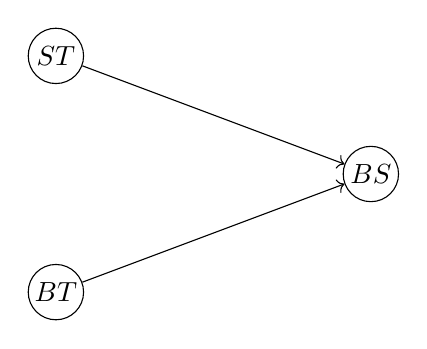
\begin{tikzpicture}
  \tikzset{vertex/.style = {shape=circle,draw,minimum size=2em,inner sep=1pt}}
  \tikzset{edge/.style = {->,- = latex'}}

	\node[vertex] (B) at (0,0) {$BT$};
	\node[vertex] (W) at (4,1.5) {$BS$};
	\node[vertex] (S) at (0,3) {$ST$};
	
       \foreach \from/\to in {B/W, S/W}
    \path[->](\from) edge node [above]{} (\to);
\end{tikzpicture}
\end{center}
\end{example}

Example \ref{ex:sym-overdetermination} is often called upon to demonstrate the concept of symmetric overdetermination. The  answer to the question, whether $ST$ the cause of $BS$, is as eluded to in \cite{hiddleston2005causal} somewhat unclear, i.e.\ some authors argue for ``yes'' and some for ``no''. However, there many of the paper considered side with declaring both $ST$ and $BT$ as causes of $BS$.
By contrast, \cite{hiddleston2005causal} embraces the ambiguous nature of this example and argues that it would be truly a victory to devise a formalisms explaining this unclairy.

%% XXXXXX Maybe example with both BT ST being required.


\begin{example}(Early Preemption)
\label{ex:backup}
Suzy throws a rock at a bottle ($ST$). The rock hits it, and the bottle shatters ($BS$). However Billy was watching Suzy, and would have thrown a rock ($BT$) just in case Suzy did not throw.
%If Trainee shoots his gun ($T$), the bullet will hit Victim ($V$). If Trainee does not shoot, Supervisor will shoot and hit Victim herself ($S$). In fact, Trainee shoots and hits Victim while Supervisor stands by.
\begin{center}
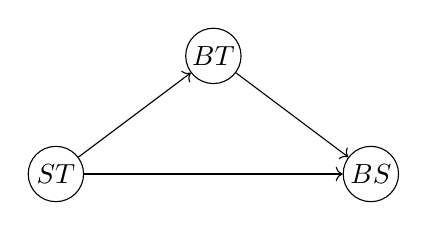
\begin{tikzpicture}
  \tikzset{vertex/.style = {shape=circle,draw,minimum size=2em,inner sep=1pt}}
  \tikzset{edge/.style = {->,- = latex'}}
	\node[vertex] (T) at (0,0) {$ST$};
	\node[vertex] (V) at (4,0) {$BS$};
	\node[vertex] (S) at (2,1.5) {$BT$};
	
       \foreach \from/\to in {T/S, T/V, S/V}
    \path[->](\from) edge node [above]{} (\to);
\end{tikzpicture}
\end{center}
\end{example}


\cite{bochman2018actual,batusov2018situation,beckers2018principled} call the phenomena in question, \emph{early preemption}.
The challenge in Example  \ref{ex:backup}  is, that the value of $BS$ does, at first glance, not depend on the value of $ST$. Because, even If $ST$ does not hold, $BT$ ensures that $BS$ remains true.
However, since Suzie's rock hit the bottle, the literature (CITE XXXX) seems to agree upon $ST$ causing $BT$. 
Interestingly, \cite{beckers2018principled} disagrees with this assessment. They argue that this scenario is virtually identical to the one in Example (XXXXSWITCH), i.e.\ $ST$ only determines how the bottle is shattered and is immaterial in determining the value of $BS$. They argue that it is the uncertainty of the processes at hand, that cause intuition to differ from Example (XXXXSWITCH).\footnote{Common alternatives use either a firing squad or assassins in their stories.}


\begin{example}(Late Preemption)
Suzy ($ST$) and Billy ($BT$) both throw rocks at a bottle, Suzy’s rock arrives first and hits the bottle ($SH$), the bottle shatters ($BS$), Billy’s arrives second and does not hit the bottle ($BH$). 
Both throws are accurate, Billy’s would have shattered the bottle if Suzy’s had not.
\begin{equation*}
\begin{split}
&BT:=1, \quad ST:= 1, \quad SH:=ST, \\
&BH:= BT \land \neg SH, \quad BS:= BH \lor SH
\end{split}
\end{equation*}
\begin{center}
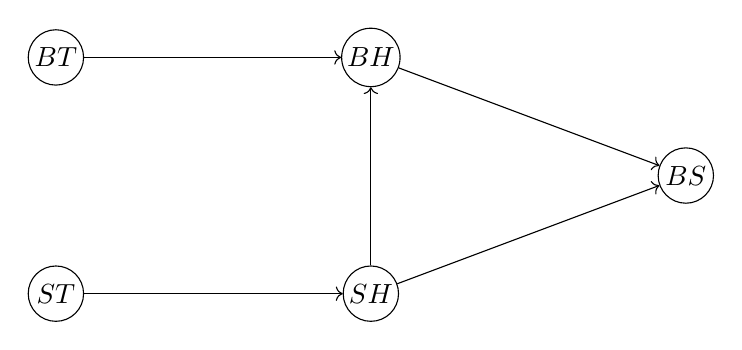
\begin{tikzpicture}
  \tikzset{vertex/.style = {shape=circle,draw,minimum size=2em,inner sep=1pt}}
  \tikzset{edge/.style = {->,- = latex'}}

  
  
	\node[vertex] (ST) at (0,0) {$ST$};
	\node[vertex] (BT) at (0,3) {$BT$};
	
	\node[vertex] (SH) at (4,0) {$SH$};
	\node[vertex] (BH) at (4,3) {$BH$};
		
	\node[vertex] (BS) at (8,1.5) {$BS$};
	
       \foreach \from/\to in {ST/SH, BT/BH, SH/BH, BH/BS, SH/BS}
    \path[->](\from) edge node [above]{} (\to);
\end{tikzpicture}
\end{center}
\end{example}







\begin{example}(Vote Machine \cite{Weslake2015partialtheory})
Two votes ($V_1$, $V_2$) are cast for a measure. The votes are summed by a machine ($M$) and the measure passes ($P$) iff it receives at least one vote.
\begin{equation*}
\begin{split}
&V_1:=1, \quad V_2:= 1 ,\\
&M:= V_1 +V_2, \quad P:= (M \geq 1)
\end{split}
\end{equation*}
\begin{center}
\begin{tikzpicture}
  \tikzset{vertex/.style = {shape=circle,draw,minimum size=2em,inner sep=1pt}}
  \tikzset{edge/.style = {->,- = latex'}}

  
  
	\node[vertex] (V1) at (0,0) {$V_1$};
	\node[vertex] (V2) at (0,3) {$V_2$};
			
	\node[vertex] (M) at (4,1.5) {$M$};
		\node[vertex] (P) at (8,1.5) {$P$};
	
       \foreach \from/\to in {V1/M, V2/M, M/P}
    \path[->](\from) edge node [above]{} (\to);
\end{tikzpicture}
\end{center}
\end{example}



\begin{example}(Loader \cite{hopkins2003clarifying,bochman2018actual,Weslake2015partialtheory}]
A firing squad consists of shooters $B$ and $C$. It is $A$’s job to load $B$’s gun, $C$ loads and fires his own gun. On a given day, $A$ loads $B$’s gun. When the time comes, only $C$ shoots the prisoner.
\begin{equation*}
\begin{split}
&A:=1, \quad B:=0, \quad C:=1 \\
&D:= (A \land B) \lor C
\end{split}
\end{equation*}
\begin{center}
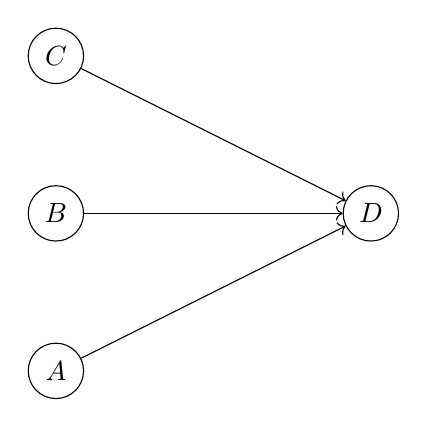
\begin{tikzpicture}
  \tikzset{vertex/.style = {shape=circle,draw,minimum size=2em,inner sep=1pt}}
  \tikzset{edge/.style = {->,- = latex'}}

  
  
	\node[vertex] (A) at (0,0) {$A$};
	\node[vertex] (B) at (0,2) {$B$};
		\node[vertex] (C) at (0,4) {$C$};
			
	\node[vertex] (D) at (4,2) {$D$};
	
       \foreach \from/\to in {A/D, B/D, C/D}
    \path[->](\from) edge node [above]{} (\to);
\end{tikzpicture}
\end{center}
\end{example}


\begin{example}(Switch \cite{Weslake2015partialtheory})
A two-state switch is wired to two lamps. If the switch is in one state ($S:=1$), only lamp one is activated ($L_1:= \neg S$), and if it is in the other state ($L_2:= S$) only lamp two is activated ($L_2=1$). In fact, lamp two is activated and the room is illuminated ($I=1$).
\begin{equation*}
\begin{split}
&S:=1\\
& L_1:= \neg S, \quad L_2:=S, \quad I:= L_1 \lor L_2
\end{split}
\end{equation*}
\begin{center}
\begin{tikzpicture}
  \tikzset{vertex/.style = {shape=circle,draw,minimum size=2em,inner sep=1pt}}
  \tikzset{edge/.style = {->,- = latex'}}

  
  
	\node[vertex] (S) at (0,1.5) {$S$};
	\node[vertex] (L1) at (4,0) {$L_1$};
		\node[vertex] (L2) at (4,3) {$L_2$};
	\node[vertex] (I) at (8,1.5) {$I$};
	
       \foreach \from/\to in {S/L1, S/L2, L1/I, L2/I}
    \path[->](\from) edge node [above]{} (\to);
\end{tikzpicture}
\end{center}
\end{example}



\begin{example}(Shock \cite{Weslake2015partialtheory})
Two two-state switches are wired to an electrode. The switches are controlled by $A$ and $B$ respectively, and the electrode is attached to $C$. $A$ has the first option to flip her switch ($A=1$). $B$ has the second option to flip her switch ($B=1$). The electrode is activated and shocks $C$ ($C=1$) iff both switches are in the same position. $B$ wants to shock $C$, and so flips her switch iff $A$ does.
\begin{equation*}
\begin{split}
&A:=1\\
& B:=A, \quad C:=(A=B)
\end{split}
\end{equation*}
\begin{center}
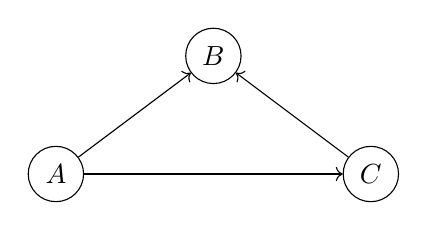
\begin{tikzpicture}
  \tikzset{vertex/.style = {shape=circle,draw,minimum size=2em,inner sep=1pt}}
  \tikzset{edge/.style = {->,- = latex'}}

  
  
	\node[vertex] (A) at (0,0) {$A$};
	\node[vertex] (B) at (2,1.5) {$B$};
	\node[vertex] (C) at (4,0) {$C$};
	
       \foreach \from/\to in {A/B, A/C, C/B}
    \path[->](\from) edge node [above]{} (\to);
\end{tikzpicture}
\end{center}
\end{example}



\begin{example}(Command  \cite{Weslake2015partialtheory})
Major ($M$) and and sergeant ($S$) stand before corporal, and both shout ‘Charge!’ ($M=1$, $S=1$). The corporal charges ($C=1$). Orders from higher- ranking soldiers trump those of lower rank, so if the major had shouted ‘Halt’ ($M=2$) the corporal would not have charged.
\begin{equation*}
\begin{split}
&M:=1, \quad S:=1\\
& C:= (M=1) \lor (S\land (M \neq 2))
\end{split}
\end{equation*}
\begin{center}
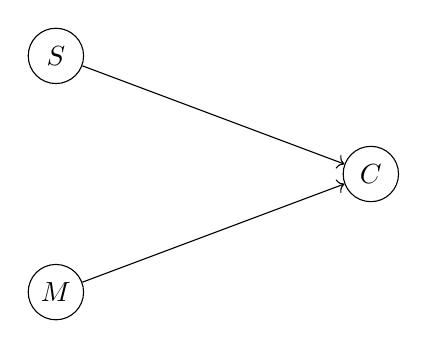
\begin{tikzpicture}
  \tikzset{vertex/.style = {shape=circle,draw,minimum size=2em,inner sep=1pt}}
  \tikzset{edge/.style = {->,- = latex'}}

  
  
	\node[vertex] (M) at (0,0) {$M$};
	\node[vertex] (S) at (0,3) {$S$};
	\node[vertex] (C) at (4,1.5) {$C$};
	
       \foreach \from/\to in {M/C, S/C}
    \path[->](\from) edge node [above]{} (\to);
\end{tikzpicture}
\end{center}
\end{example}


\begin{example}(Combinatorial Lamp  \cite{Weslake2015partialtheory})
A lamp ($L$) is controlled by three switches ($A$, $B$ and $C$), each of which has three possible positions ($-1$, $0$, $1$). The lamp switches on iff two or more switches are in the same position. In fact, the switches are in positions $A=1$, $B=-1$ and $C=-1$.
\begin{equation*}
\begin{split}
&A:=1, \quad B:=-1, \quad C:=-1\\
& L:= (A=B) \lor (B=C) \lor (A=C)
\end{split}
\end{equation*}
\begin{center}
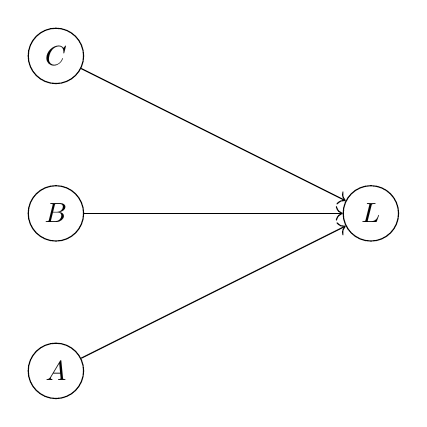
\begin{tikzpicture}
  \tikzset{vertex/.style = {shape=circle,draw,minimum size=2em,inner sep=1pt}}
  \tikzset{edge/.style = {->,- = latex'}}

  
  
	\node[vertex] (A) at (0,0) {$A$};
	\node[vertex] (B) at (0,2) {$B$};
		\node[vertex] (C) at (0,4) {$C$};
			
	\node[vertex] (L) at (4,2) {$L$};
	
       \foreach \from/\to in {A/L, B/L, C/L}
    \path[->](\from) edge node [above]{} (\to);
\end{tikzpicture}
\end{center}
\end{example}


\begin{example}(Careful Antidote  \cite{Weslake2015partialtheory})
Assassin is in possession of a lethal poison, but has a last-minute change of heart and refrains from putting it in Victim’s coffee ($A=0$). Bodyguard puts antidote in the coffee ($B=1$), which would have neutralized the poison. Victim drinks the coffee and survives ($D=0$).
\begin{equation*}
\begin{split}
&A:=0, \quad B:=1 \\
&D:= A\land \neg B
\end{split}
\end{equation*}
\begin{center}
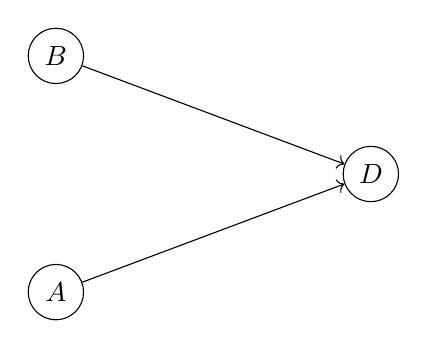
\begin{tikzpicture}
  \tikzset{vertex/.style = {shape=circle,draw,minimum size=2em,inner sep=1pt}}
  \tikzset{edge/.style = {->,- = latex'}}

  	\node[vertex] (A) at (0,0) {$A$};
	\node[vertex] (B) at (0,3) {$B$};
	\node[vertex] (D) at (4,1.5) {$D$};
	
       \foreach \from/\to in {A/D, B/D}
    \path[->](\from) edge node [above]{} (\to);
  

\end{tikzpicture}
\end{center}
\end{example}


\begin{example}(Careful Poisoning \cite{Weslake2015partialtheory})
Assistant Bodyguard puts a harmless antidote in Victim’s coffee ($A=1$). Buddy then poisons the coffee ($B=1$), using a poison that is normally lethal, but which is countered by the antidote. Buddy would not have poisoned the coffee if Assistant had not administered the antidote first. Victim drinks the coffee and survives ($D=0$).
\begin{equation*}
\begin{split}
&A:=1 \\
&B:=A, \quad D:=\neg A \land B
\end{split}
\end{equation*}
\begin{center}
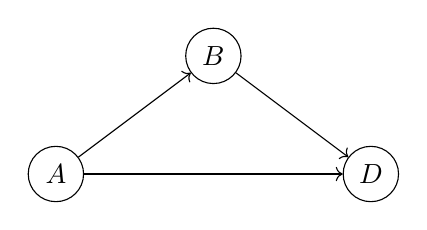
\begin{tikzpicture}
  \tikzset{vertex/.style = {shape=circle,draw,minimum size=2em,inner sep=1pt}}
  \tikzset{edge/.style = {->,- = latex'}}

  
  
	\node[vertex] (A) at (0,0) {$A$};
	\node[vertex] (B) at (2,1.5) {$B$};
	\node[vertex] (D) at (4,0) {$D$};
	
       \foreach \from/\to in {A/B, B/D, A/D}
    \path[->](\from) edge node [above]{} (\to);
\end{tikzpicture}
\end{center}
\end{example}


\begin{example}(Careful Poisoning \cite{Weslake2015partialtheory})
I push($P=1$) Jones in front of a truck ($T=1$),which hits ($H=1$) and kills him ($D=1$); if I had not done so ($P=0$), a bus ($B=1$) would have hit ($H=1$) and killed him.
\begin{itemize}
\item[(i)] There is no other action available.
\item[(ii)] I can push ($P = 2$) Jones to safety ($H = 0$).
\end{itemize}

\begin{equation*}
\begin{split}
&P:=1, \quad T:=1, \quad B:=1\\
&H:=(P=1 \land T=1) \lor (P=0 \land B=1), \quad D:=H
\end{split}
\end{equation*}
\begin{center}
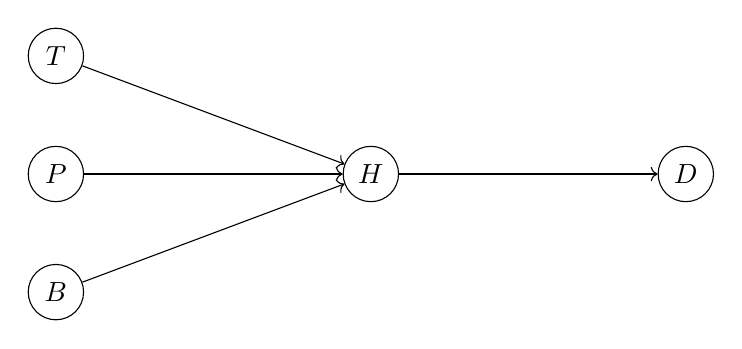
\begin{tikzpicture}
  \tikzset{vertex/.style = {shape=circle,draw,minimum size=2em,inner sep=1pt}}
  \tikzset{edge/.style = {->,- = latex'}}

  
  
	\node[vertex] (B) at (0,0) {$B$};
	\node[vertex] (P) at (0,1.5) {$P$};
	\node[vertex] (T) at (0,3) {$T$};
	
	
	\node[vertex] (H) at (4,1.5) {$H$};
	\node[vertex] (D) at (8,1.5) {$D$};
	
       \foreach \from/\to in {B/H, T/H, P/H, H/D}
    \path[->](\from) edge node [above]{} (\to);
\end{tikzpicture}
\end{center}
\end{example}




\begin{example}(Careful Poisoning \cite{Weslake2015partialtheory})
A lamp ($L$) is controlled by three switches ($A$, $B$ and $C$), each of which has three possible positions ($-1$, $0$, $1$). The switches are connected to detectors ($N_{-1}$, $N_0$, $N_1$), each of which is activated iff no switch is in position ($-1$, $0$, $1$) respectively. The lamp switches on iff some detector is activated. In fact, the switches are in positions $A=1$, $B=-1$ and $C=-1$, detector $N_0$ is activated, and $L=1$.


\begin{equation*}
\begin{split}
&A:=1, B:=-1, C:=-1\\
&N_{-1}:=\neg (A=-1 \lor B=-1 \lor C=-1) \\
&N_{0}:=\neg (A=0 \lor B=0 \lor C=0) \\
&N_{1}:=\neg (A=1 \lor B=1 \lor C=1) \\
&L:= N_{-1} \lor N_0 \lor N_1 \\
\end{split}
\end{equation*}
\begin{center}
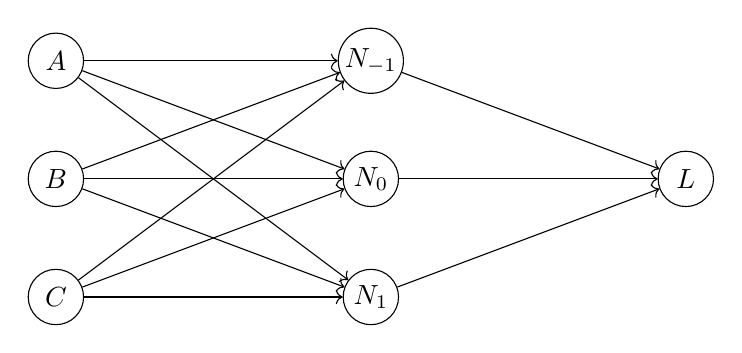
\begin{tikzpicture}
  \tikzset{vertex/.style = {shape=circle,draw,minimum size=2em,inner sep=1pt}}
  \tikzset{edge/.style = {->,- = latex'}}

  
  
	\node[vertex] (A) at (0,0) {$C$};
	\node[vertex] (B) at (0,1.5) {$B$};
	\node[vertex] (C) at (0,3) {$A$};
	
		\node[vertex] (N-1) at (4,0) {$N_{1}$};
	\node[vertex] (N0) at (4,1.5) {$N_0$};
	\node[vertex] (N1) at (4,3) {$N_{-1}$};

	\node[vertex] (L) at (8,1.5) {$L$};
	
       \foreach \from/\to in {A/N1, A/N0, A/N-1,B/N1, B/N0, B/N-1,C/N1, C/N0,C/N-1, N-1/L, N0/L, N1/L}
    \path[->](\from) edge node [above]{} (\to);
\end{tikzpicture}
\end{center}
\end{example}



\subsection{Summary}
\begin{table}[]
\begin{tabular}{ | c | c | c | c | c | c | c |}
\hline 
& \cite{batusov2018situation} & \cite{beckers2018principled} & \cite{bochman2018actual}  & \cite{hiddleston2005causal} & \cite{hitchcock2007three}  & \cite{Weslake2015partialtheory}  \\
\hline 
Backup & &  &  &  &  &  1 \\
Window  & &  &  &  &  &  1 \\
Bottle  & &  &  &  &  &  1 \\
Vote Machine  & &  &  &  &  &  1 \\
Loader  & &  &  &  &  &  1 \\
Switch  & &  &  &  &  &  1 \\
Shock  & &  &  &  &  &  1 \\
Command  & &  &  &  &  &  1 \\
Combination Lamp  & &  &  &  &  &  1 \\
Careful Antidote  & &  &  &  &  &  1 \\
Careful Poisoning & & &  &  &  &   1 \\
Push  & &  &  &  &  &  1 \\
Fancy Lamp  & &  &  &  &  &  1 \\
\hline 
\end{tabular}
\end{table}

\chapter{Computational Causality}

\section{Modelling Languages}

To introduce some of the languages used to encode causal relationships a simple example is required. 
\begin{example}
\label{ex:causal_model_forrest_fire_1}
Consider the following causal relation:
\begin{itemize}
\item Both a lightning strike ($\mathit{LS}$) or a dropped match ($\mathit{MD}$) can to cause a forest fire ($\mathit{FF}$).
\end{itemize}
\end{example}

\begin{example}
\label{ex:causal_model_forrest_fire_2}
Consider the following causal relation:
\begin{itemize}
\item Both a lightning strike ($\mathit{LS}$) and a dropped match ($\mathit{MD}$) are required to cause a forest fire ($\mathit{FF}$).
\end{itemize}
%Was the forest fire ($\mathit{FF}$) caused by an arsonist dropping a lit match ($\mathit{MD}$), or be a lightning strike ($\mathit{LS}$).
\end{example}

\begin{example}
\label{ex:causal_model_forrest_fire_3}
Consider the following causal relations:
\begin{itemize}
\item A small fire ($\mathit{SF}$) causes a big fire ($\mathit{BF}$).
\item A big fire ($\mathit{BF}$) causes a forest fire ($\mathit{FF}$).
\item A thunderstorm ($\mathit{TS}$) causes rain fall ($\mathit{RF}$) and lightning strikes ($\mathit{LS}$).
\item Lightning  ($\mathit{LS}$) strikes cause big fires  ($\mathit{BS}$)
\item Rainfall ($\mathit{RF}$) prevents small fires ($\mathit{SF}$).  
\item Dropping a match ($\mathit{MD}$) causes a small fire ($\mathit{SF}$)
\end{itemize}
%Given a clear sky ($\mathit{CS}$), was the forest fire ($\mathit{FF}$) caused by an arsonist dropping a lit match ($\mathit{MD}$), or be a lightning strike ($\mathit{LS}$).
%Both a lightning strike or the dropped match can cause the forest fire. However, no lightning can occur if the sky is blue. 
\end{example}

\subsection{Neural Diagrams}
\label{sec:neural_diagrams}
In the more philosophical literature \emph{neuron diagrams} are commonly used to encode token causal relations, thus assisting the structural exploration of various examples concerned with token causation \cite{baumgartner2013regularity,erwig2010causal}. 
In their simplest form a neuron diagram can be understood as a directed acyclic graph, where each vertex, called neuron, can either fire or not, often indicated by its color. A neuron can be either \emph{exogenous}, i.e. it has no incoming edges, or \emph{endogenous}, i.e. it has at least one incoming edge. Moreover, edges between neurons can also be separated into two categories, i.e. \emph{stimulating} edges and \emph{inhibiting} edges, often distinguished trough having a triangle and respectively a circle as arrow head. 
In its simplest form such neuron diagrams follow a fairly straight forward semantic. That is, while it is externally specified whether an exogenous neuron fires of not, an endogenous neuron fires if and only if it is stimulated by at least one firing neuron, and inhibited by zero firing neurons \cite{hitchcock2009structural,erwig2010causal,baumgartner2013regularity}. 

\begin{example}
Consider Example \ref{ex:causal_model_forrest_fire_3}. Assume that $\mathit{MD}$ and $\mathit{TS}$ fire. This results in the following diagram.
\begin{center}
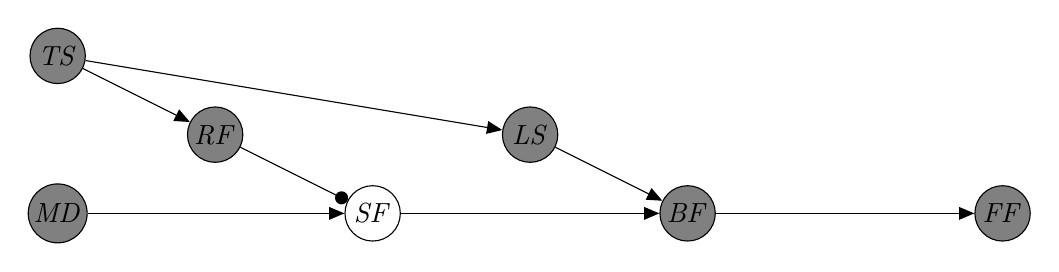
\begin{tikzpicture}
  \tikzset{neuron/.style = {shape=circle,draw,minimum size=2em,inner sep=1pt}}
    \tikzset{fireneuron/.style = {shape=circle,draw,minimum size=2em,inner sep=1pt, fill=gray}}
  \tikzset{edge/.style = {->,> = latex'}}
  \tikzset{%
  tipA/.tip={Triangle[angle=45:6pt]},
}

	\node[fireneuron] (MD) at (0,0) {$\mathit{MD}$};
	
	\node[neuron] (SF) at (4,0) {$\mathit{SF}$};
	\node[fireneuron] (BF) at (8,0) {$\mathit{BF}$};
	\node[fireneuron] (FF) at (12,0) {$\mathit{FF}$};
	
	\node[fireneuron] (TS) at (0,2) {$\mathit{TS}$};
	\node[fireneuron] (LS) at (6,1) {$\mathit{LS}$};
	\node[fireneuron] (RF) at (2,1) {$\mathit{RF}$};
	
	
	 \path[-*] (RF) edge node [above]{} (SF);
	 
    \foreach \from/\to in {MD/SF, SF/BF, BF/FF, TS/LS, TS/RF, LS/BF}
    \path[-tipA](\from) edge node [above]{} (\to);

\end{tikzpicture}
\end{center}
Here it is clear to see that $\mathit{TS}$ and $\mathit{MD}$ are exogenous, while the remaining are endogenous. Moreover, the effect of $\mathit{MD}$ is cancelled, due to the fact that $\mathit{RF}$ fired.
\end{example}


The previous example, only used one kind of neuron. However, this would be insufficient to capture many examples, e.g.\ such a restriction makes modelling of Example \ref{ex:causal_model_forrest_fire_2} already problematic.
Hence, as for example demonstrated in \cite{hitchcock2009structural} and \cite{baumgartner2013regularity}, alternative, more complicated neurons can be introduced. For example, one could consider a stubborn neuron that only fires, if all of its predecessors fire as well, or a neuron that only fires if the number of stimulating inputs is greater that the number of inhibiting inputs.

\begin{example}
Consider Example \ref{ex:causal_model_forrest_fire_2}. If one considers $\mathit{FF}$ to be a stubborn neuron, i.e.\ one that only fires, if all of its predecessors fire, then the causal relations presented can be encoded as the following neuron diagram.
\begin{center}
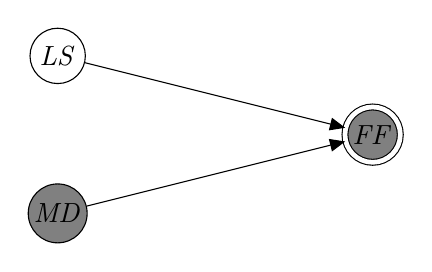
\begin{tikzpicture}
  \tikzset{neuron/.style = {shape=circle,draw,minimum size=2em,inner sep=1pt}}
    \tikzset{fireneuron/.style = {shape=circle,draw,minimum size=2em,inner sep=1pt, fill=gray}}
    \tikzset{stubbornneuron/.style = {shape=circle,draw,minimum size=2em,inner sep=1pt, double, double distance=0.6mm}}
    \tikzset{firestubbornneuron/.style = {shape=circle,draw,minimum size=2em,inner sep=1pt, fill=gray,double, double distance=0.6mm}}
  \tikzset{edge/.style = {->,> = latex'}}
  \tikzset{%
  tipA/.tip={Triangle[angle=45:6pt]},
}
	
	\node[fireneuron] (MD) at (0,0) {$\mathit{MD}$};
	\node[neuron] (LS) at (0,2) {$\mathit{LS}$};
	\node[firestubbornneuron] (FF) at (4,1) {$\mathit{FF}$};

    \foreach \from/\to in {MD/FF, LS/FF}
    \path[-tipA](\from) edge node [above]{} (\to);

\end{tikzpicture}
\end{center}
\end{example}

%
%The intuition conveyed above was both formalised and generalised in \cite{erwig2010causal}. To do so they destination between \emph{neuron graphs} capturing an abstract neuron structure and \emph{neuron diagrams} representing the execution of neuron graphs for some set of inputs. 
%For the subsequent definitions, let $\mathbb{F}_{\mathbb{B}}^{k,m}:= \{f \mid f:\mathbb{B}^k\to \mathbb{B}^m\}$ be the set of functions mapping $k$ boolean inputs to $m$ boolean outputs. 
%Let $\cbinfoos := \bigcup_{k>0} \mathbb{F}_{\mathbb{B}}^{k,1}$ be the set of all boolean functions. 

%\begin{definition}[\cite{erwig2010causal}]
%A \emph{neuron graph} is a directed acyclic graph $\ngraph:=(\cvars, \crel,\kappa, \sigma_{\cenvars})$, where $\cvars$ is the set of neurons and can be partitioned into endogenous variables $\cenvars$ and exogenous variables $\cexvars$; $\crel$ is a set of edges; $\kappa:V \to \{\text{§},!\}$ labels a neuron as either law or action; $\sigma_{\cenvars}:=\{ \sigma_v \mid \forall v \in \cenvars \; \sigma_v : \gtpred(v) \to \mathbb{B}\}$ is a set of functions mapping the predecessors of endogenous variables to a binary value.
%
% $\sigma_{\cenvars} : \cenvars \to \{f \mid f: \gtpred(v) \to \mathbb{B}\}$ maps every endogenous variable to an appropriate boolean function, i.e. for every $v \in \cenvars$ one has $\sigma_{\cenvars}(v): \cbinfoos^{\gtdegpred(v)} \to \mathbb{B}$. For $v \in \cvars$ let $\pi(v)$ be predefined ordering over $\gtpred(v)$.
%\end{definition}
%
%Moreover, from this one can build a neuron diagram by taking a neuron graph and providing an assignment of the exogenous variables.
%
%\begin{definition}[\cite{erwig2010causal}]
%Let $\ngraph:=(\cvars, \crel,\kappa, \sigma)$ be a neuron graph, then $\ndiagram:= (\ngraph, \sigma_{\cexvars}) $ is a \emph{neuron diagram} with  $\sigma_{\cexvars}: \cexvars \to \mathbb{B}$, i.e. 
%\end{definition}
%
%To evaluate such a neuron diagram, a firing semantic is required. 
%
%\begin{definition}[\cite{erwig2010causal}]




The intuition conveyed above was both formalised and generalised in \cite{erwig2010causal}. To do so they destination between \emph{neuron graphs} capturing an abstract neuron structure and \emph{neuron diagrams} representing the execution of neuron graphs for some set of inputs. For the subsequent definitions, let $\mathbb{F}_{\mathbb{B}}^{k,m}:= \{f \mid f:\mathbb{B}^k\to \mathbb{B}^m\}$ be the set of functions mapping $k$ boolean inputs to $m$ boolean outputs. 
Let $\cbinfoos := \bigcup_{k>0} \mathbb{F}_{\mathbb{B}}^{k,1}$ be the set of all boolean functions. 

\begin{definition}
A \emph{neuron graph} is a directed acyclic graph $\ngraph:=(\cvars, \crel, \cfoos, \pi)$, where $\cvars$ is the set of neurons and can be partitioned into endogenous variables $\cenvars$ and exogenous variables $\cexvars$; $\crel$ is a set of edges; 
 $\cfoos:=\{ F_v \mid \forall v \in \cenvars \; F_v : \cbinfoos^{\gtdegpred(v)} \to \mathbb{B} \}$ is a set of boolean functions;  for $v \in \cvars$ let $\pi(v):= (v_1,\dots, v_n) $ an ordering of $\gtpred(v)$.
%$\sigma_{\cenvars} : \cenvars \to \cbinfoos$ maps every endogenous variable to an appropriate boolean function, i.e. for every $v \in \cenvars$ one has $\sigma_{\cenvars}(v): \cbinfoos^{\gtdegpred(v)} \to \mathbb{B}$.
\end{definition}

Moreover, from this one can build a neuron diagram by taking a neuron graph and providing an assignment of the exogenous variables.

\begin{definition}
Let $\ngraph:=(\cvars, \crel, \cfoos, \pi)$ be a neuron graph, then $\ndiagram:= (\ngraph,\sigma)$ is a \emph{neuron diagram} and 
$\sigma : \cexvars \to \mathbb{B}$ being an assignment mapping exogenous variables to binary values.
%$\sigma :=\{ \sigma_v \mid \forall v \in \cexvars \;  \sigma_v \in \cbinfoos^{0,1}\}$ being a set of constant binary functions.
\end{definition}

To evaluate such a neuron diagram, a firing semantic is required. Intuitively, an endogenous neuron $v$ fires, if and only if the assigned boolean function evaluates to $1$ given the values of its predecessors ordered based on the ordering $\pi(v)$. Being assigned a constant function and having no predecessors, this recursive process ends at an exogenous node.

\begin{definition}
Let $\ndiagram:=(\ngraph,\sigma) $ be a neuron diagram, then $\interi$ is defined such that $\forall v \in \cvars$ and for $\pi(v)=(v_1, \dots, v_n)$
\begin{equation*}
\interi(v):= 
\begin{cases}
\sigma(v) & \quad \text{if} \; v \in \cexvars \\
F_v(\mathcal{I}(v_1), \dots , \mathcal{I}(v_n)) & \quad \text{if} \; v \in \cenvars
\end{cases}
\end{equation*}
(As a shorthand let $\interi(v):= \sigma_v(\mathcal{I}(v_1), \dots , \mathcal{I}(v_n))$.)
\end{definition}


In \cite{erwig2010causal} this generalised form of neuron diagrams is used to construct a formalism that can be used for causal inference (see XXXXXX). This, however, requires a slight extension of the definition.

\begin{definition}
A \emph{labelled neuron graph} is a directed acyclic graph $\ngraph:=(\cvars, \crel, \cfoos, \pi, \kappa)$ where  $\ngraph:=(\cvars, \crel, \cfoos, \pi)$  is a neuron graph and $\kappa:\cvars \to \{\text{§},!\}$ marks a neuron as either law or action. 
\end{definition}

A \emph{labelled neuron diagram} is simply builds upon a labelled neuron graph, rather than a mere neuron graph.


Reasoning with such structures was for example critiqued by Hitchcock \cite{hitchcock2009structural} of failing in encoding complex relationships between variables, he supports the causal model approach relying on structural equations presented in Section  \ref{sec:causal_models}. 
This was even acknowledged in \cite{erwig2010causal}, citing the simplicity of neuron diagrams (graphs) to justify their usefulness. 





%For purpose of this section, neural diagrams will be used as a useful method for striping the examples presented in this section down to their bare structure, permitting a clear comparison of the formalisms presented in Chapter \ref{ch:comp_causality}, based on which neurons they deem causal for the firing of another. 


\subsection{Causal Models}
\label{sec:causal_models}
One common method for encoding the causal structure of a problem, especially when dealing with counterfactual approaches in the context of token causality, are \emph{Causal Models}, i.e. they encode counterfactual relationships between variables. While such causal models have their origin in \cite{pearl1995causal}, the version introduced, taken from \cite{halpern2015cause}, was formulated in \cite{halpern2000axiomatizing}. However, \cite{Weslake2015partialtheory} slightly changed the notation to make the direction of such structural equations more apparent, thus this convention will be carried over into this work \cite{halpern2015cause,Weslake2015partialtheory}. 


The idea underlying causal models is that the world can be described by a set of random variables and a set of deterministic, structural equations. 
By contrast, approaches such as Causal Bayesian Networks (see XXXXX) are inherently probabilistic. In  \cite{pearl2009causality} compares those two approaches by drawing an analogy to the Laplacian and the quantum mechanical conception of physics. That is, the prior considers natures laws as deterministic and uncertainty only emerges due to ignorance, while the latter understands determinism as a mere approximation of inherently probabilistic laws.
However, as the goal of this endeavour is to capture the understanding of causality intuitive to humans, the focus on the prior is apt \cite{pearl2009causality}. 
In \cite{halpern2015cause} Halpern introduces structural models using the following example.

\begin{example}
\label{ex:causal_model_forrest_fire}
Consider Example \ref{ex:causal_model_forrest_fire_1}  and Example \ref{ex:causal_model_forrest_fire_2}.
In both cases the variables are considered as binary random variables, e.g.\ if $\mathit{FF} = 1$ then the forest fire occurred, if $\mathit{FF} = 0$ it did not.
For the prior the causal relationship is encoded by the structural equation $\mathit{FF} = \max(\mathit{LS}, \mathit{MD})$, while for the latter the structural equation $\mathit{FF} = \min(\mathit{LS}, \mathit{MD})$
can be used.
\end{example}

Be not mistaken, a structural equation are best read as assignments rather than as a algebraic equation. Meaning that the value of the dependent variable, in this case $\mathit{FF}$, can not influence the values of the variables determining its values, in this case $\mathit{MD}$ and $\mathit{LS}$. As eluded to earlier, in this example the temptation of imposing a probabilistic relationship between values becomes apparent, e.g.\ it is tempting say that if a lighting strikes there is a probability of $0.8$ of a forest fire occurring. Similarly to Pearl, Haplern advises against such relations, suggesting instead two alternative approaches. Firstly, expand the model such that this uncertainty can be described, e.g.\ adding variables such as dryness or altitude. Secondly, he suggest, one could push all relevant factors into a single variable $U$, e.g.\ this variable would explain all the conditions required for the lightning to strike or the arsonist to drop their match.  Moreover, the utility of $U$ can be further expanded upon, by allowing it to encode the relation between values, in this case it determines the value of $\mathit{FF}$ by allowing $U$ to determine the structural equation used, e.g.\ $\min$ or $\max$. As in Subsection \ref{subsec:neural_diagrams}, the variables of an causal model can be split into exogenous and endogenous variables. Depending on whether $U$ was used or not, either $U$ is exogenous and $\mathit{LS}$, $\mathit{MD}$ and $\mathit{FF}$ are endogenous or $\mathit{LS}$  and $\mathit{MD}$ exogenous and $\mathit{FF}$ is endogenous. Using the now cultivated intuition a formal definition can be given \cite{halpern2015cause}.
 

\begin{definition}[\cite{halpern2015cause}]
A \emph{causal model} $\cmodel:=(\csig, \cfoos)$ is a pair, where $\csig$ is a signature and $\cfoos$ is a set of modifiable structural equations.
A signature $\csig:=(\cexvars, \cenvars, \crange)$ is a tuple, where $\cexvars$ is a set of exogenous variables, $\cenvars$ is a set of endogenous variables and $\crange$ is a function mapping 
a variable $Y \in \cvars$ ($:=\cexvars \cup \cenvars$) to a set containing all possible values of $Y$. 
$\cfoos$ maps each variable $X\in \cenvars$ to a function $F_X:  \bigtimes_{Y \in \cvars\setminus \{X\}} \crange(Y) \to \crange(X)$.
\end{definition}

While never explicitly stated, the definition of $F_X$ requires some order imposed onto the variables in $\cvars$. To prevent unnecessary and cumbersome notational overload, such an approach will be followed in this work as well.
More often than not, the function $F_X$ will be expressed using a short hand notation. That is, for the causal model $\cmodel$ where $\cexvars := \{U\}$ and $\cenvars := \{Y,Y',X\}$, the function $F_{X}(Y,Y'U):=Y+U$ is abbreviated
as $X = Y+U$. To emphasise that this structural equation not an equation in the classical algebraic sense \cite{Weslake2015partialtheory} writes it as assignment $X := Y+U$.
Moreover, if $\forall x \in \cvars\; \crange(x)=\mathbb{B}$ then one speaks of an \emph{binary causal model}.

Emerging out of the counterfactual tradition, it is natural that the language provides a convenient method to express \emph{interventions}. That is, given a causal model $\cmodel:=(\csig, \cfoos)$, the model $\cmodel_{X \leftarrow x}:=(\csig, \cfoos_{X \leftarrow x})$ where $\cfoos_{X \leftarrow x}$ is identical to $\cfoos$, but for the structural equation of $X$ which will be fixed to $X:=x$.


Computing the values of the variables present in an causal model requires \emph{context}, i.e.\ an assignment of values to all exogenous variables. From there, one can compute the values of all endogenous variables, by solving the respective equations.

\begin{definition}
Given a causal model $\cmodel:=(\csig, \cfoos)$ and an assignment $\sigma$ where for $u \in \cexvars$ $\sigma(u) \in \crange(u)$, then $(\cmodel, \sigma)$ is a causal model with context.
\end{definition}

In general, such causal models could have cyclic relationships among their variables. However, so called \emph{acyclic} causal models tend to be the primary subject of investigation, which considering the context of token causality, seems to be a sensible decision. Moreover, due to the fact that in an acyclic model the value of an endogenous variable is uniquely determined given the values of the exogenous variables, it allows for simpler reasoning. Intuitively, a causal model is considered acyclic, if one can order the endogenous variables such that a variable can not be influenced be the values of the variables above \cite{halpern2015cause}.  

\begin{definition}[\cite{halpern2015cause}]
Let $\cmodel$ be a causal model, $\cmodel$ is \emph{acyclic} (or \emph{recursive}) if $X$ is independent $Y$, i.e.\ there exists a total ordering $\prec$ of $\cenvars$ such that
\begin{equation*}
 X \prec Y \implies  \forall y,y' \in \crange(Y) \; F_X(\dots , y, \dots) = F_X(\dots , y', \dots) 
\end{equation*}
\end{definition}

Relying on its acyclicity one can easily compute the values of the variables in a recursive fashion, by starting with the context, then iteratively assigning those variables their values that have structural equations relying only on already computed values. This can be continued until all variables are assigned a value, i.e.\ until a fixed point is reached.



As discussed in XXXX, there are some examples, termed \emph{non-structural counterexamples}, which suggest that a certain notion of normality is required to properly model certain causal relations.
This can be accomplished by considering multiple world, some more normal than others. That is, by encoding ones intuition of normality using a partial pre-order\footnote{A partial pre-order is a reflexive and transitive relation} $\succeq$, a world $s$, characterised by an assignment of values to the exogenous variables, can be considered as least as normal as the world $s'$, iff $s \succeq s'$ \cite{halpern2015cause}.

\begin{definition}[\cite{halpern2015cause}]
The tuple $\cmodel:= (\csig, \cfoos, \succeq)$ is called an extended causal model, iff $(\csig, \cfoos)$ is a causal model and $\succeq$ is a pre-order over worlds. A
world $s$ being $s \in   \bigtimes_{U \in \cexvars} \crange(U)$.
\end{definition}


Such extended causal models provide a high degree of modelling power. Such power generates certain advantages, such as allowing one to capture the distinction between conditions and causes present in the legal tradition of causality, with conditions being simply values of variables with a higher degree of normality. However, it also provides the modeller with the ability to render many causal semantics irrelevant, thus further exacerbating Hall's complaint\footnote{The structural equations approach places a much greater emphasis on problem modelling, amounting to little more than building the solution into the model \cite{erwig2010causal}} about the structural equation approach. 

\subsection{Causal Calculus}



\subsection{Situation Calculus}


\subsection{CP-Logic}



\chapter{Analysis}

\section{Expressivity}


While the unified notation used across multiple formalisms is intended to promote understanding, by allowing the transfer of previously obtained concepts, it may be confusing when directly comparing said formalisms.
Therefore, a superscript indicating the membership of a certain object will be used to mitigate this pitfall. 


COMMENT: maybe work with $y$  and $y'$.


Intuitively, the following transformation, takes each exogenous (endogenous) neuron and transforms it into an exogenous (endogenous) variable for a causal model. The binary function assigned to endogenous neurons will be assigned to the corresponding endogenous variables in the causal model. And an assignment to exogenous variables, will be carried over to corresponding exogenous variables as well. 


\begin{definition}
%Let $\tau_{G\to M}$ be a function transforming a neuron graph into a binary acyclic causal model.
Let neuron graph $\ngraph:=(\cvars^{\ngraph}, \crel^{\ngraph}, \cfoos^{\ngraph}, \pi^{\ngraph})$, then $\tau_{G\to M}(\ngraph)=\cmodel:=(\csig^{\cmodel}, \cfoos^{\cmodel})$ is the causal model:
\begin{itemize}
\item $\csig^{\cmodel}:=(\cexvars^{\cmodel}, \cenvars^{\cmodel}, \crange^{\cmodel})$ where $\cexvars^{\cmodel}$ is a set of variables such that each $U^{\cmodel} \in \cexvars^{\cmodel}$ corresponds with a single neuron in $u^{\ngraph} \in \cexvars^{\ngraph}$; where $\cenvars^{\cmodel}$ is a set of variables such that each $V^{\cmodel} \in \cenvars^{\cmodel}$ corresponds with a single neuron in $v^{\ngraph} \in \cenvars^{\ngraph}$; 
where $\forall x^{\ngraph} \in \cvars^{\ngraph} \; \crange(X^{\cmodel})=\mathbb{B}$.
\item $\forall x^{\ngraph} \in \cenvars^{\ngraph}$ and for  $\pi^{\ngraph}(x^{\ngraph})=(y_1^{\ngraph}, \dots, y_n^{\ngraph} )$,  $F_{X}^{\cmodel}(\overline{W}):= F_{x}^{\ngraph}(Y_1^{\cmodel} , \dots , Y_n^{\cmodel})$ 
where $\overline{W}$ is the tuple form of $\cvars \setminus \{X\}$ (according to some implicit order).
\end{itemize}
Let $\sigma^{\ngraph}$ be an assignment for $\ngraph$ then $\sigma^{\cmodel} := \tau_{G\to M}(\sigma^{\ngraph})$ where $\forall u^{\ngraph} \in \cexvars^{\ngraph} \sigma^{\cmodel}(U^{\cmodel}):=\sigma^{\ngraph}(u^{\ngraph})$ is a context for $ \cmodel=\tau_{G\to M}(\ngraph)$.
\end{definition}

The resulting causal model is clearly binary. Moreover, by taking the transitive closure of $\crel$ one obtains a partial order, which then can be extended to a total order using the order-extension principle (see \cite{felgner1999independence}) one obtains a total order that complies with the partial order, i.e. if $x \leq y$ in the partial order then $x \leq y$ in the total order. 
Now with the equations form the neuron graph being carried over, it is easy to see that the resulting total order demonstrates that the causal model is in fact acyclic. (FORMALISE??)


\begin{lemma}
Given an arbitrary neuron graph $\ngraph$ and an arbitrary assignment $\sigma^{\ngraph}$ for $\ngraph$. Then for the causal model $\cmodel:=\tau_{G\to M}(\ngraph)$ and the assignment $\sigma^{\cmodel}:= \tau_{G\to M}\sigma^{\ngraph})$ it holds that
$\forall x^{\ngraph} \in \cvars^{\ngraph} \; X^{\cmodel} = \interi(x^{\ngraph})$.
\end{lemma}
\begin{proof}
This can be demonstrated by using induction over the number of computation steps.
In the base case, the only variables determined are those assigned by $\sigma^{\cmodel}$. Here one can observe that
$\forall x^{\ngraph} \in \cexvars^{\ngraph} \; X^{\cmodel} =  \sigma^{\cmodel}(X^{\cmodel})  =  \sigma^{\ngraph}(x^{\ngraph})= \interi(x^{\ngraph})$.
Acyclicity ensures that every value computed during the $n+1^{\text{th}}$ computation step, requires only previously derived values. By induction, it must be that for all those values
$ X^{\cmodel} = \interi(x^{\ngraph})$ holds. Now take an arbitrary variable considered in the $n+1^{\text{th}}$ computation step. Its value is determined using the same equation used for determining whether the corresponding neuron fires. Furthermore, the induction hypothesis it is ensured that the input values for this function are identical. Hence, this implies that this particular variable must have the same value as its corresponding neuron. (FORMALISE !!!!)
\end{proof}


MISSING
\begin{definition}
%Let $\tau_{G\to M}$ be a function transforming a neuron graph into a binary acyclic causal model.
Let $\cmodel:=(\csig^{\cmodel}, \cfoos^{\cmodel})$ be a binary acyclic causal model, then $\tau_{M\to G}(\cmodel):=(\cvars^{\ngraph}, \crel^{\ngraph}, \cfoos^{\ngraph}, \pi^{\ngraph})$ is the neuron graph:
\begin{itemize}
\item $\cvars^{\ngraph} $ is a set of neurons, where each variable $X^{\cmodel}$ has a corresponding neuron  $x^{\ngraph} \in \cvars^{\ngraph} $;
\item  $(x^{\ngraph}, y^{\ngraph}) \in \crel^{\ngraph}$ if $x^{\cmodel}$ influences $y^{\cmodel}$, i.e. $\exists y^{\cmodel},y'^{\cmodel} \in \cvars^{\cmodel}$ \\
$F_{X}^{\cmodel}(\dots , y^{\cmodel}, \dots ) \neq F_{X}^{\cmodel}(\dots , y'^{\cmodel}, \dots)$.
\item For some $X^{\cmodel} \in \cvars^{\cmodel}$,  $\pi(x^{\ngraph})$ is the tuple created from $\cvars^{\ngraph} \cap \gtpred(x^{\ngraph})$ by sorting them according to the implied order of the corresponding variables over $\cvars^{\cmodel}$.
\item $\cfoos^{\ngraph}$ is the set of function $F_x^{\ngraph}$ is the binary function obtained from $F_X^{\cmodel}$ by reducing its domain to those variables 
\end{itemize}
\end{definition}


\chapter{Literature Review}

\section{Methodology}
\label{sec:methodology}

It is vital to build an adequate repository of papers upon which this survey shall draw upon. Inherent in this construction is the tension between scope and depth, as all else equal, one compromises the other. Positioning a survey on this spectrum in a justifiable manner is rather difficult. Therefore, the scope of this survey shall be determined by rigorously adhering to the mechanics of reproducible methodology. This approach is an attempt to alleviate the temptation of individually justifying why a certain paper was selected or discarded. 

The methodology underlying this systematic literature review employs a snowball search strategy to construct its set of relevant papers. 
In general, according to \cite{wohlin2014guidelines} any snowball search strategy should construct a start set and employ forward and backward snowballing at each iteration to construct the final set of papers. 
Moreover, starting set should satisfied the following criteria.
\begin{itemize}
\item The start set should cover a diversity of communities, especially if they may from independent cluster.
\item The number of papers in the start set should not be too small.
\item The number of papers in the start set should not be too big.
\item The start set should cover several different publishers, years and authors.
\item The start set ought to be formulated from keywords (and their synonyms) in the research question.
\end{itemize}
Furthermore, using this start set the final set of papers is constructed iteratively by employing backward snowballing, i.e.\ for every unprocessed paper add all relevant references to the set of papers, and forward snowballing, i.e.\ for every unprocessed paper use Google Scholar to identify every relevant paper citing the current article \cite{wohlin2014guidelines}. Using this as a template, the actual methodology is constructed accordingly.


Firstly, reproducibility being a primary objective the notion of relevancy requires special attention, i.e.
\begin{definition}
A paper is \emph{potentially relevant} (within the context of literature search), if
\begin{itemize}
\item  its title contains a word starting with the characters \emph{``caus''} or 
\item  its abstract contains a word starting with the characters \emph{``causal''}. 
\end{itemize}
\end{definition}
%Those criteria where selected as ``caus'' can easily be extended to causes, causal, causality, causing, etc. 
Obviously this criteria may lead to some unnecessary considerations. Hence, if a paper classified as potentially relevant is deemed irrelevant under closer inspection, it will discarded. All remaining papers will be considered as relevant. 
\begin{definition}
A paper is \emph{relevant}, if it is potentially relevant and not irrelevant.  
\end{definition}
Unfortunately, the the notion or irrelevance can not be properly defined. Precisely because of this, one is able to use it to prevent unnecessary exploration. However, to ensure transparency, the classification of any potentially relevant paper as irrelevant, will be argued for on a case by case basis in the Appendix \ref{ch:appendix}.

Secondly, ACCESSIBILITY


Thirdly, to further ensure reproducibility any dynamic tools for search (e.g.\ results of literature search engines, number of citations) must be rejected, thus prohibiting the application of forward snowballing. To compensate for this, the start set is constructed accordingly, i.e.
\begin{definition}
The \emph{start set} contains every relevant and accessible paper published in 
\begin{itemize}
\item \href{https://www.journals.elsevier.com/knowledge-based-systems}{Journal Knowledge-Bases Systems}
\item \href{https://www.journals.elsevier.com/artificial-intelligence}{Journal Artificial Intelligence}
\item \href{https://www.springer.com/journal/10506}{Journal Artificial Intelligence and Law}
\item \href{https://www.ijcai.org/}{International Joint Conferences on Artificial Intelligence Organization}
\end{itemize}
between 01.01.2017 and 31.1.2019.
\end{definition}
Being primarily concerned with publications discussing causality within the context of artificial intelligence, with possible applications in law, this starting set should provide a sufficient strong directive.
Moreover, due to the fact that forward snowballing will not be employed, only very recent publications will be considered.

Fourthly, as eluded to earlier, an iteration consists only of backwards snowballing.
\begin{definition}
The function $\mathit{snowball}$ maps a paper $x$ to the set containing every relevant and accessible paper cited by $x$.
\end{definition}


Lastly, the following characterisation of the paper repository can be constructed.
\begin{definition}
Let $\mathfrak{P}_0$ be the start set, and let $\mathfrak{P}_{n+1}=\mathfrak{P}_{n} \cup \{x \mid \forall y \in \mathfrak{P}_{n} \; x \in \mathit{snowball}(y) \}$, i.e. the set of papers after $n+1$ iterations is constructed by adding all papers obtained through snowballing over the set of papers after $n$ iterations to said set.
\end{definition}

%!!!No books but book chapters !!!!
\section{Paper Repository}

Using the methodology outlined in Section \ref{sec:methodology} the start set contains $37$ papers, i.e. 




%
%\chapter{Computational Causality}
%\label{ch:comp_causality}
%\begin{quote}
%But what's really hard about this area, I'm going to give you a definition and I would love to be able to prove a theorem that says ``this is the right definition''. I'm a theoretician that's what I do. I prove theorems. If I only knew the statement of the theorem I might have a shot of proving it, but I don't know what it means to have the right definition of causality. [\dots] I don't know what the theorem should say and so what's traditional in the literature [\dots]
%%and frankly what I'll be doing as well 
%is the philosophers and the lawyers have come up with hundreds of examples and the way you show your definition is good is to show that ``gee look at how well it does it all in all the examples'' and that works fine until somebody comes along and constructs an example to show your definition maybe wasn't as good as you thought it was [\dots].
%\end{quote}
%
%


%
%
%
%


%##################################################################################################################
%
%\chapter*{Appendix}
%\label{ch:appendix}
%
%
%
%\section{Notation}
%
%\begin{itemize}
%\item $\cvars$ set of variables;
%\item $\cenvars$ set of endogenous variables;
%\item $\cexvars$ set of exogenous variables;
%\item $\crel$ set of causal relations;
%\item $\mathbb{F}_{\mathbb{B}}^{k,m}:= \{f \mid f:\mathbb{B}^k\to \mathbb{B}^m\}$ is set of functions mapping $k$ boolean inputs to $m$ boolean outputs;
%\item $\mathbb{F}_{\mathbb{B}} := \bigcup_{k>0} \mathbb{F}_{\mathbb{B}}^{k,1}$ is the set of all boolean functions;
%\end{itemize}
%
%
%
%
%
%
%\section{Examples}
%
%\begin{example}(Backup \cite{Weslake2015partialtheory})
%If Trainee shoots his gun ($T$), the bullet will hit Victim ($V$). If Trainee does not shoot, Supervisor will shoot and hit Victim herself ($S$). In fact, Trainee shoots and hits Victim while Supervisor stands by.
%\begin{equation*}
%\begin{split}
%&T := 1, \quad S:= \neg T, \\
%& V := T \lor S
%\end{split}
%\end{equation*}
%\begin{center}
%\begin{tikzpicture}
%  \tikzset{vertex/.style = {shape=circle,draw,minimum size=2em,inner sep=1pt}}
%  \tikzset{edge/.style = {->,- = latex'}}
%
%  
%  
%	\node[vertex] (T) at (0,0) {$T$};
%	\node[vertex] (V) at (4,0) {$V$};
%	\node[vertex] (S) at (2,1.5) {$S$};
%	
%       \foreach \from/\to in {T/S, T/V, S/V}
%    \path[->](\from) edge node [above]{} (\to);
%\end{tikzpicture}
%\end{center}
%\end{example}
%
%
%\begin{example}(Window \cite{Weslake2015partialtheory})
%Billy ($B=1$) and Suzy ($S=1$) both throw rocks at a window, each with sufficient force to shatter it. The rocks strike the window at exactly the same time. The window breaks ($W=1$).
%\begin{equation*}
%\begin{split}
%&S:=1 , \quad B:=1, \\
%& W:= B \lor S
%\end{split}
%\end{equation*}
%\begin{center}
%\begin{tikzpicture}
%  \tikzset{vertex/.style = {shape=circle,draw,minimum size=2em,inner sep=1pt}}
%  \tikzset{edge/.style = {->,- = latex'}}
%
%  
%  
%	\node[vertex] (B) at (0,0) {$B$};
%	\node[vertex] (W) at (4,1.5) {$W$};
%	\node[vertex] (S) at (0,3) {$S$};
%	
%       \foreach \from/\to in {B/W, S/W}
%    \path[->](\from) edge node [above]{} (\to);
%\end{tikzpicture}
%\end{center}
%\end{example}
%
%
%\begin{example}(Bottle \cite{Weslake2015partialtheory})
%Suzy ($ST$) and Billy ($BT$) both throw rocks at a bottle, Suzy’s rock arrives first and hits the bottle ($SH$), the bottle shatters ($BS$), Billy’s arrives second and does not hit the bottle ($BH$). 
%Both throws are accurate, Billy’s would have shattered the bottle if Suzy’s had not.
%\begin{equation*}
%\begin{split}
%&BT:=1, \quad ST:= 1, \quad SH:=ST, \\
%&BH:= BT \land \neg SH, \quad BS:= BH \lor SH
%\end{split}
%\end{equation*}
%\begin{center}
%\begin{tikzpicture}
%  \tikzset{vertex/.style = {shape=circle,draw,minimum size=2em,inner sep=1pt}}
%  \tikzset{edge/.style = {->,- = latex'}}
%
%  
%  
%	\node[vertex] (ST) at (0,0) {$ST$};
%	\node[vertex] (BT) at (0,3) {$BT$};
%	
%	\node[vertex] (SH) at (4,0) {$SH$};
%	\node[vertex] (BH) at (4,3) {$BH$};
%		
%	\node[vertex] (BS) at (8,1.5) {$BS$};
%	
%       \foreach \from/\to in {ST/SH, BT/BH, SH/BH, BH/BS, SH/BS}
%    \path[->](\from) edge node [above]{} (\to);
%\end{tikzpicture}
%\end{center}
%\end{example}
%
%
%\begin{example}(Vote Machine \cite{Weslake2015partialtheory})
%Two votes ($V_1$, $V_2$) are cast for a measure. The votes are summed by a machine ($M$) and the measure passes ($P$) iff it receives at least one vote.
%\begin{equation*}
%\begin{split}
%&V_1:=1, \quad V_2:= 1 ,\\
%&M:= V_1 +V_2, \quad P:= (M \geq 1)
%\end{split}
%\end{equation*}
%\begin{center}
%\begin{tikzpicture}
%  \tikzset{vertex/.style = {shape=circle,draw,minimum size=2em,inner sep=1pt}}
%  \tikzset{edge/.style = {->,- = latex'}}
%
%  
%  
%	\node[vertex] (V1) at (0,0) {$V_1$};
%	\node[vertex] (V2) at (0,3) {$V_2$};
%			
%	\node[vertex] (M) at (4,1.5) {$M$};
%		\node[vertex] (P) at (8,1.5) {$P$};
%	
%       \foreach \from/\to in {V1/M, V2/M, M/P}
%    \path[->](\from) edge node [above]{} (\to);
%\end{tikzpicture}
%\end{center}
%\end{example}
%
%
%
%\begin{example}(Loader \cite{Weslake2015partialtheory})
%A firing squad consists of shooters $B$ and $C$. It is $A$’s job to load $B$’s gun, $C$ loads and fires his own gun. On a given day, $A$ loads $B$’s gun. When the time comes, only $C$ shoots the prisoner.
%\begin{equation*}
%\begin{split}
%&A:=1, \quad B:=0, \quad C:=1 \\
%&D:= (A \land B) \lor C
%\end{split}
%\end{equation*}
%\begin{center}
%\begin{tikzpicture}
%  \tikzset{vertex/.style = {shape=circle,draw,minimum size=2em,inner sep=1pt}}
%  \tikzset{edge/.style = {->,- = latex'}}
%
%  
%  
%	\node[vertex] (A) at (0,0) {$A$};
%	\node[vertex] (B) at (0,2) {$B$};
%		\node[vertex] (C) at (0,4) {$C$};
%			
%	\node[vertex] (D) at (4,2) {$D$};
%	
%       \foreach \from/\to in {A/D, B/D, C/D}
%    \path[->](\from) edge node [above]{} (\to);
%\end{tikzpicture}
%\end{center}
%\end{example}
%
%
%\begin{example}(Switch \cite{Weslake2015partialtheory})
%A two-state switch is wired to two lamps. If the switch is in one state ($S:=1$), only lamp one is activated ($L_1:= \neg S$), and if it is in the other state ($L_2:= S$) only lamp two is activated ($L_2=1$). In fact, lamp two is activated and the room is illuminated ($I=1$).
%\begin{equation*}
%\begin{split}
%&S:=1\\
%& L_1:= \neg S, \quad L_2:=S, \quad I:= L_1 \lor L_2
%\end{split}
%\end{equation*}
%\begin{center}
%\begin{tikzpicture}
%  \tikzset{vertex/.style = {shape=circle,draw,minimum size=2em,inner sep=1pt}}
%  \tikzset{edge/.style = {->,- = latex'}}
%
%  
%  
%	\node[vertex] (S) at (0,1.5) {$S$};
%	\node[vertex] (L1) at (4,0) {$L_1$};
%		\node[vertex] (L2) at (4,3) {$L_2$};
%	\node[vertex] (I) at (8,1.5) {$I$};
%	
%       \foreach \from/\to in {S/L1, S/L2, L1/I, L2/I}
%    \path[->](\from) edge node [above]{} (\to);
%\end{tikzpicture}
%\end{center}
%\end{example}
%
%
%
%\begin{example}(Shock \cite{Weslake2015partialtheory})
%Two two-state switches are wired to an electrode. The switches are controlled by $A$ and $B$ respectively, and the electrode is attached to $C$. $A$ has the first option to flip her switch ($A=1$). $B$ has the second option to flip her switch ($B=1$). The electrode is activated and shocks $C$ ($C=1$) iff both switches are in the same position. $B$ wants to shock $C$, and so flips her switch iff $A$ does.
%\begin{equation*}
%\begin{split}
%&A:=1\\
%& B:=A, \quad C:=(A=B)
%\end{split}
%\end{equation*}
%\begin{center}
%\begin{tikzpicture}
%  \tikzset{vertex/.style = {shape=circle,draw,minimum size=2em,inner sep=1pt}}
%  \tikzset{edge/.style = {->,- = latex'}}
%
%  
%  
%	\node[vertex] (A) at (0,0) {$A$};
%	\node[vertex] (B) at (2,1.5) {$B$};
%	\node[vertex] (C) at (4,0) {$C$};
%	
%       \foreach \from/\to in {A/B, A/C, C/B}
%    \path[->](\from) edge node [above]{} (\to);
%\end{tikzpicture}
%\end{center}
%\end{example}
%
%
%
%\begin{example}(Command  \cite{Weslake2015partialtheory})
%Major ($M$) and and sergeant ($S$) stand before corporal, and both shout ‘Charge!’ ($M=1$, $S=1$). The corporal charges ($C=1$). Orders from higher- ranking soldiers trump those of lower rank, so if the major had shouted ‘Halt’ ($M=2$) the corporal would not have charged.
%\begin{equation*}
%\begin{split}
%&M:=1, \quad S:=1\\
%& C:= (M=1) \lor (S\land (M \neq 2))
%\end{split}
%\end{equation*}
%\begin{center}
%\begin{tikzpicture}
%  \tikzset{vertex/.style = {shape=circle,draw,minimum size=2em,inner sep=1pt}}
%  \tikzset{edge/.style = {->,- = latex'}}
%
%  
%  
%	\node[vertex] (M) at (0,0) {$M$};
%	\node[vertex] (S) at (0,3) {$S$};
%	\node[vertex] (C) at (4,1.5) {$C$};
%	
%       \foreach \from/\to in {M/C, S/C}
%    \path[->](\from) edge node [above]{} (\to);
%\end{tikzpicture}
%\end{center}
%\end{example}
%
%
%\begin{example}(Combinatorial Lamp  \cite{Weslake2015partialtheory})
%A lamp ($L$) is controlled by three switches ($A$, $B$ and $C$), each of which has three possible positions ($-1$, $0$, $1$). The lamp switches on iff two or more switches are in the same position. In fact, the switches are in positions $A=1$, $B=-1$ and $C=-1$.
%\begin{equation*}
%\begin{split}
%&A:=1, \quad B:=-1, \quad C:=-1\\
%& L:= (A=B) \lor (B=C) \lor (A=C)
%\end{split}
%\end{equation*}
%\begin{center}
%\begin{tikzpicture}
%  \tikzset{vertex/.style = {shape=circle,draw,minimum size=2em,inner sep=1pt}}
%  \tikzset{edge/.style = {->,- = latex'}}
%
%  
%  
%	\node[vertex] (A) at (0,0) {$A$};
%	\node[vertex] (B) at (0,2) {$B$};
%		\node[vertex] (C) at (0,4) {$C$};
%			
%	\node[vertex] (L) at (4,2) {$L$};
%	
%       \foreach \from/\to in {A/L, B/L, C/L}
%    \path[->](\from) edge node [above]{} (\to);
%\end{tikzpicture}
%\end{center}
%\end{example}
%
%
%\begin{example}(Careful Antidote  \cite{Weslake2015partialtheory})
%Assassin is in possession of a lethal poison, but has a last-minute change of heart and refrains from putting it in Victim’s coffee ($A=0$). Bodyguard puts antidote in the coffee ($B=1$), which would have neutralized the poison. Victim drinks the coffee and survives ($D=0$).
%\begin{equation*}
%\begin{split}
%&A:=0, \quad B:=1 \\
%&D:= A\land \neg B
%\end{split}
%\end{equation*}
%\begin{center}
%\begin{tikzpicture}
%  \tikzset{vertex/.style = {shape=circle,draw,minimum size=2em,inner sep=1pt}}
%  \tikzset{edge/.style = {->,- = latex'}}
%
%  	\node[vertex] (A) at (0,0) {$A$};
%	\node[vertex] (B) at (0,3) {$B$};
%	\node[vertex] (D) at (4,1.5) {$D$};
%	
%       \foreach \from/\to in {A/D, B/D}
%    \path[->](\from) edge node [above]{} (\to);
%  
%
%\end{tikzpicture}
%\end{center}
%\end{example}
%
%
%\begin{example}(Careful Poisoning \cite{Weslake2015partialtheory})
%Assistant Bodyguard puts a harmless antidote in Victim’s coffee ($A=1$). Buddy then poisons the coffee ($B=1$), using a poison that is normally lethal, but which is countered by the antidote. Buddy would not have poisoned the coffee if Assistant had not administered the antidote first. Victim drinks the coffee and survives ($D=0$).
%\begin{equation*}
%\begin{split}
%&A:=1 \\
%&B:=A, \quad D:=\neg A \land B
%\end{split}
%\end{equation*}
%\begin{center}
%\begin{tikzpicture}
%  \tikzset{vertex/.style = {shape=circle,draw,minimum size=2em,inner sep=1pt}}
%  \tikzset{edge/.style = {->,- = latex'}}
%
%  
%  
%	\node[vertex] (A) at (0,0) {$A$};
%	\node[vertex] (B) at (2,1.5) {$B$};
%	\node[vertex] (D) at (4,0) {$D$};
%	
%       \foreach \from/\to in {A/B, B/D, A/D}
%    \path[->](\from) edge node [above]{} (\to);
%\end{tikzpicture}
%\end{center}
%\end{example}
%
%
%\begin{example}(Careful Poisoning \cite{Weslake2015partialtheory})
%I push($P=1$) Jones in front of a truck ($T=1$),which hits ($H=1$) and kills him ($D=1$); if I had not done so ($P=0$), a bus ($B=1$) would have hit ($H=1$) and killed him.
%\begin{itemize}
%\item[(i)] There is no other action available.
%\item[(ii)] I can push ($P = 2$) Jones to safety ($H = 0$).
%\end{itemize}
%
%\begin{equation*}
%\begin{split}
%&P:=1, \quad T:=1, \quad B:=1\\
%&H:=(P=1 \land T=1) \lor (P=0 \land B=1), \quad D:=H
%\end{split}
%\end{equation*}
%\begin{center}
%\begin{tikzpicture}
%  \tikzset{vertex/.style = {shape=circle,draw,minimum size=2em,inner sep=1pt}}
%  \tikzset{edge/.style = {->,- = latex'}}
%
%  
%  
%	\node[vertex] (B) at (0,0) {$B$};
%	\node[vertex] (P) at (0,1.5) {$P$};
%	\node[vertex] (T) at (0,3) {$T$};
%	
%	
%	\node[vertex] (H) at (4,1.5) {$H$};
%	\node[vertex] (D) at (8,1.5) {$D$};
%	
%       \foreach \from/\to in {B/H, T/H, P/H, H/D}
%    \path[->](\from) edge node [above]{} (\to);
%\end{tikzpicture}
%\end{center}
%\end{example}
%
%
%
%
%\begin{example}(Careful Poisoning \cite{Weslake2015partialtheory})
%A lamp ($L$) is controlled by three switches ($A$, $B$ and $C$), each of which has three possible positions ($-1$, $0$, $1$). The switches are connected to detectors ($N_{-1}$, $N_0$, $N_1$), each of which is activated iff no switch is in position ($-1$, $0$, $1$) respectively. The lamp switches on iff some detector is activated. In fact, the switches are in positions $A=1$, $B=-1$ and $C=-1$, detector $N_0$ is activated, and $L=1$.
%
%
%\begin{equation*}
%\begin{split}
%&A:=1, B:=-1, C:=-1\\
%&N_{-1}:=\neg (A=-1 \lor B=-1 \lor C=-1) \\
%&N_{0}:=\neg (A=0 \lor B=0 \lor C=0) \\
%&N_{1}:=\neg (A=1 \lor B=1 \lor C=1) \\
%&L:= N_{-1} \lor N_0 \lor N_1 \\
%\end{split}
%\end{equation*}
%\begin{center}
%\begin{tikzpicture}
%  \tikzset{vertex/.style = {shape=circle,draw,minimum size=2em,inner sep=1pt}}
%  \tikzset{edge/.style = {->,- = latex'}}
%
%  
%  
%	\node[vertex] (A) at (0,0) {$C$};
%	\node[vertex] (B) at (0,1.5) {$B$};
%	\node[vertex] (C) at (0,3) {$A$};
%	
%		\node[vertex] (N-1) at (4,0) {$N_{1}$};
%	\node[vertex] (N0) at (4,1.5) {$N_0$};
%	\node[vertex] (N1) at (4,3) {$N_{-1}$};
%
%	\node[vertex] (L) at (8,1.5) {$L$};
%	
%       \foreach \from/\to in {A/N1, A/N0, A/N-1,B/N1, B/N0, B/N-1,C/N1, C/N0,C/N-1, N-1/L, N0/L, N1/L}
%    \path[->](\from) edge node [above]{} (\to);
%\end{tikzpicture}
%\end{center}
%\end{example}
%
%
%
%
%
%
%
%
%
%
%
%
%
%\begin{example}
%A traveler goes on a trip through the desert and takes a bottle of water. Two people try to kill the traveler: the first poisons the water while the second pokes a hole in the bottle. On the trip the traveler gets thirsty, tries to drink from the bottle, finds it empty, and dies of de- hydration.
%
%\end{example}
%%\begin{itemize}
%%\item \cite{verheij2017proof} This paper is deemed not relevant, as it is primarily concerned with the averaging of baysian networks and its application to law, than with causality. Here the notion of causality only enters the picture in form of an example subcategory of baysian networks, i.e. causal networks.
%%\item \cite{zhang2017characterizing} Alternative article was chosen \cite{zhang2015characterizing}
%%\item \cite{constantinou2017towards} Does not seem relevant, unsure.
%%\end{itemize} 
%

\printbibliography

\end{document}

%
%\begin{center}
%\begin{tikzpicture}
%  \tikzset{vertex/.style = {shape=circle,draw,minimum size=2em,inner sep=1pt}}
%  \tikzset{edge/.style = {-,- = latex'}}
%  
%  
%  
%	\node[vertex] (00)[label=right:$\models \varphi_*(2)$ ; $\models \varphi_*(3)$]  at (5,4) {$0,0$};
%	\node[vertex] (21) at (2,6.5) {$2,1$};
%	\node[vertex] (22) at (3.5,6.5) {$2,2$};
%	\node[vertex] (23) [label=below:$\models \neg p$] at (5,6.5) {$2,3$};
%	\node[vertex] (24) [label=below:$\models \varphi(2)$] at (6.5,6.5) {$2,4$};
%	\node[vertex] (25) [label=below:$\models \neg p$] at (8,6.5) {$2,5$};
%	\node[vertex] (26) [label=below:$p$]  at (9.5,6.5) {$2,6$};
%	
%	\node[vertex] (31) at (0.5,1.5) {$3,1$};
%	\node[vertex] (32) at (2,1.5) {$3,2$};
%	\node[vertex] (33) at (3.5,1.5) {$3,3$};
%	\node[vertex] (34) [label=below:$\models \neg p$] at (5,1.5) {$3,4$};
%	\node[vertex] (35) [label=below:$\models \neg p$] at (6.5,1.5) {$3,5$};
%	\node[vertex] (36) [label=below:$\models \varphi(3)$] at (8,1.5) {$3,6$};
%	\node[vertex] (37) [label=below:$\models \neg p$] at (9.5,1.5) {$3,7$};
%	\node[vertex] (38) [label=below:$\models \neg p$] at (11,1.5) {$3,8$};
%	\node[vertex] (39)  [label=below:$p$] at (12.5,1.5) {$3,9$};
%
%    \foreach \from/\to in {00/21,21/31,22/23,24/25, 00/31, 32/33, 34/35, 36/37, 38/39}
%    \path[-](\from) edge node [above]{$a$} (\to);
%
%       \foreach \from/\to in {21/22,23/24,25/26, 31/32, 33/34, 35/36, 37/38}
%    \path[-](\from) edge node [above]{$b$} (\to);
%\end{tikzpicture}
%\end{center}
